\documentclass[dvipdfmx]{jarticle}
\usepackage{graphicx}
\usepackage{amsmath}
\usepackage[top=30truemm,bottom=30truemm,left=25truemm,right=25truemm]{geometry}
\usepackage{listings,jvlisting}

\lstset{
  basicstyle={\ttfamily},
  identifierstyle={\small},
  commentstyle={\smallitshape},
  keywordstyle={\small\bfseries},
  ndkeywordstyle={\small},
  stringstyle={\small\ttfamily},
  frame={tb},
  breaklines=true,
  columns=[l]{fullflexible},
  numbers=left,
  xrightmargin=0zw,
  xleftmargin=3zw,
  numberstyle={\scriptsize},
  stepnumber=1,
  numbersep=1zw,
  lineskip=-0.5ex
}

\begin{document}

\begin{titlepage}
    \begin{center}
        \vspace*{60pt}
        {\LARGE プログラミングDレポート}
        \vspace*{240pt}\\
        \begin{tabular}{rl}
            担当教員 & 小南大智\\
            提出日 & \today\\
            氏名 & 山久保孝亮\\
            学籍番号 & 09B22084\\
            メールアドレス & u327468b@ecs.osaka-u.ac.jp
        \end{tabular}
    \end{center}
\end{titlepage}

\section{プログラムの操作方法と機能}
今回のライフゲームの課題はRunボタンが押されるとゲームが開始する.
私が作成した機能と操作方法は以下のとおりである.
\subsection{盤面の描画}
今回のライフゲームではゲームが開始した際にウィンドウが開き,そこにnext,undo,newgameのボタンとともに盤面が表示されるという仕様になっている.
盤面のサイズの初期値は縦300,横400ピクセルで最小値は縦,横である.生きている状態のセルを黒色,死んでいる状態のセルを灰色で表すこととした.最初はすべてのセルが死んでいる状態となっている.
また,盤面の縦と横の座標は以下の図1ような仕様とした.これは,(i,j)と指定されると横軸がi,縦軸がjの行と列をそれぞれ考え,それらが交差するセルを表す.
\begin{figure}[h]
  \centering
  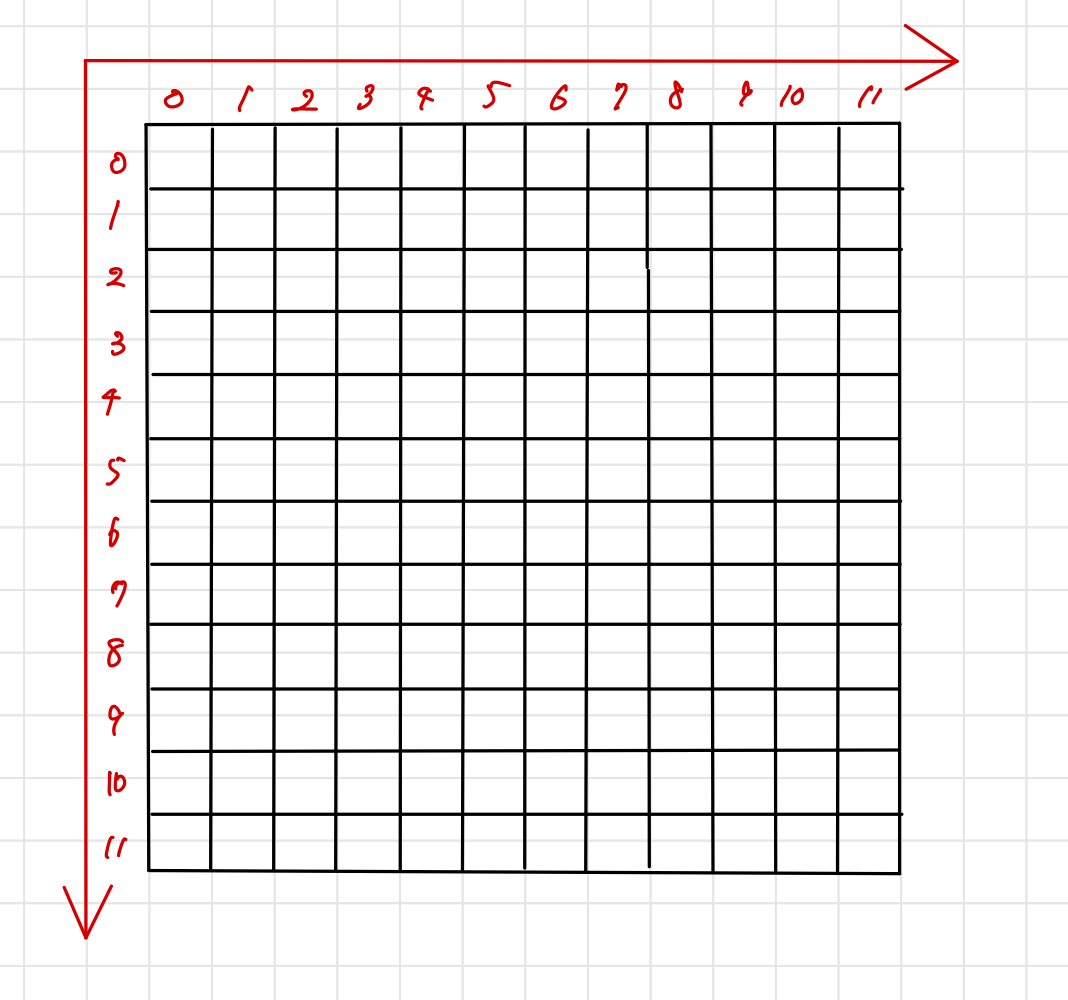
\includegraphics[width=6cm]{zahyou.png}
  \caption{座標の仕様}
\end{figure}
\subsubsection{ウィンドウのサイズ変更}
ウィンドウの大きさをユーザ側が変更した際にはその変更に合わせて盤面の大きさも変更される.
以下の図2はMainクラス内のコードの一部である.赤く囲んだ部分の数字は縦のセルの個数,青く囲んだ部分の数字は横のセルの個数を表す.
ユーザはこの部分のコードを変更して盤面の個数を変更することができる.
\begin{figure}[h]
  \centering
  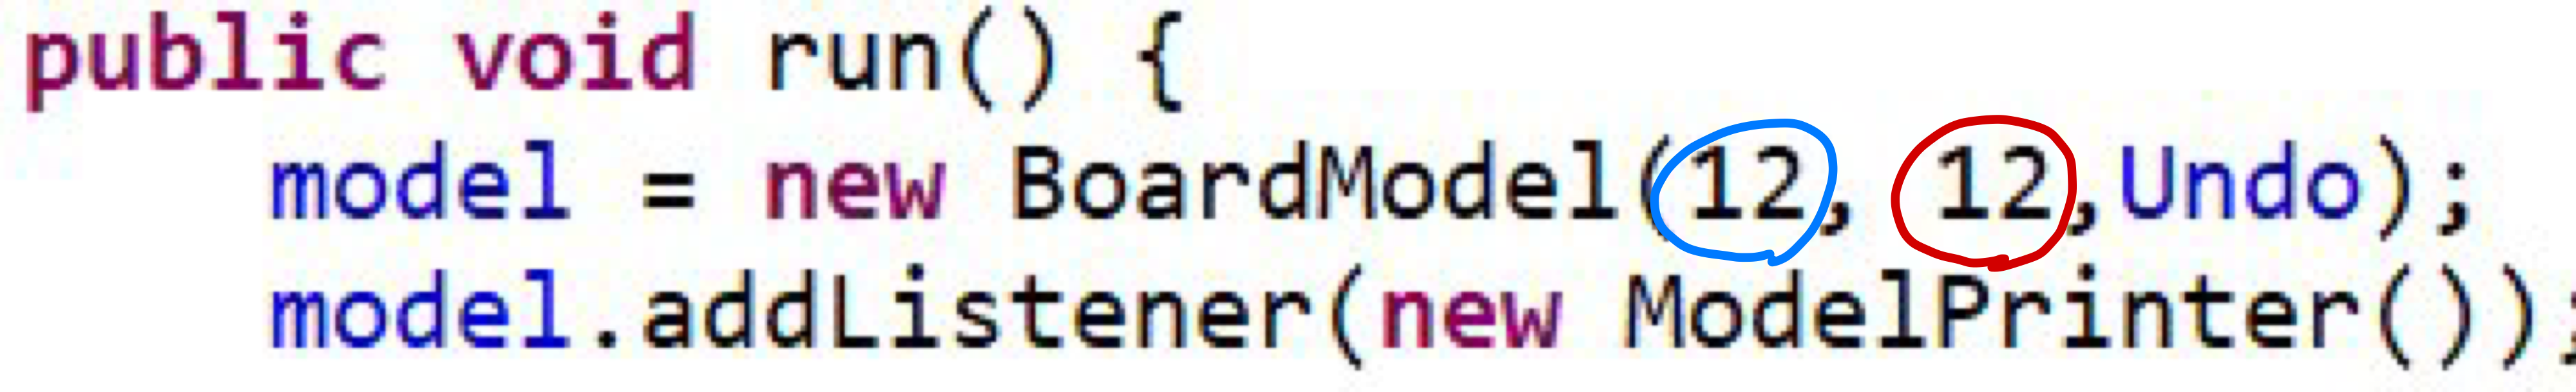
\includegraphics[width=6cm]{code_masu.png}
  \caption{該当部分のコード}
\end{figure}
\\ただしセルの形は常に正方形を保つ.
パネル上にボタンを表示させる範囲を確保してから,そこを除いた部分に盤面を描写する.具体的な盤面内の座標の計算は実現方法のところで記述する.
以下の図2,3はウィンドウを極端に横に大きくしたときの例と縦に大きくしたときの例である.
\begin{figure}[htbp]
    \begin{minipage}[b]{0.45\linewidth}
      \centering
      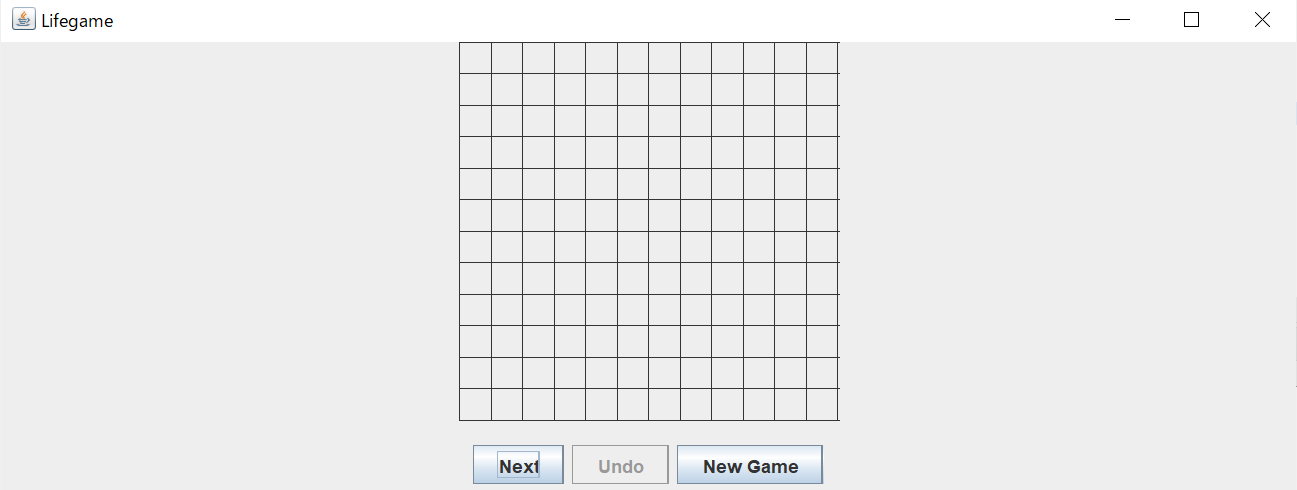
\includegraphics[keepaspectratio, scale=0.3]{wide.png}
      \caption{極端に横に大きくしたときの盤面}
    \end{minipage}
    \begin{minipage}[b]{0.45\linewidth}
      \centering
      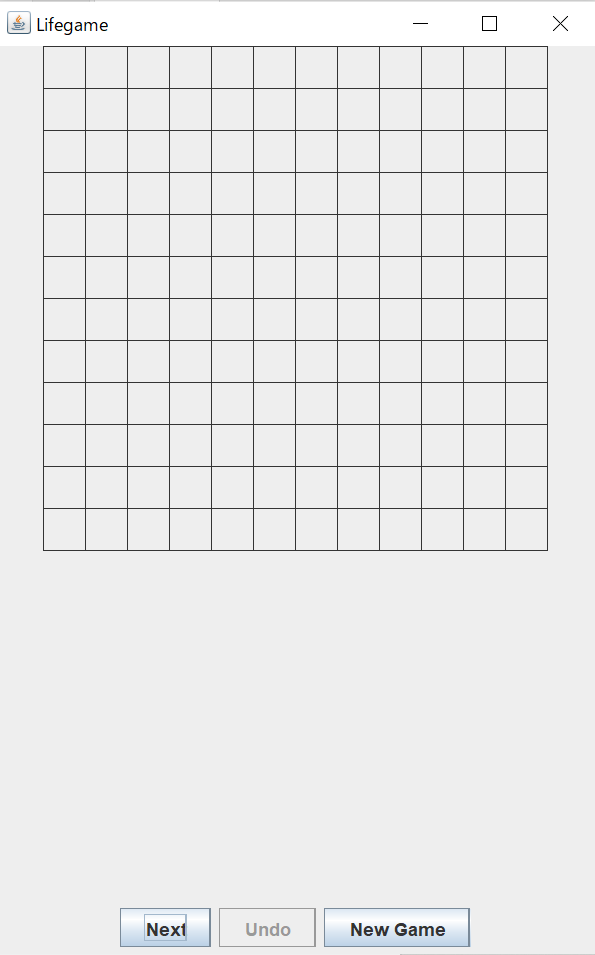
\includegraphics[keepaspectratio, scale=0.3]{height.png}
      \caption{極端に縦に大きくしたときの盤面}
    \end{minipage}
  \end{figure}
\subsubsection{盤面のサイズ変更}
盤面はそれぞれのセルの正方形がMainクラスで初期化されたセルの数だけそれぞれ縦と横に表示される.
以下の4,5はRUNボタンを押して出力した$12\times12$と$18\times12$の盤面である.
\begin{figure}[htbp]
  \begin{minipage}[b]{0.45\linewidth}
    \centering
    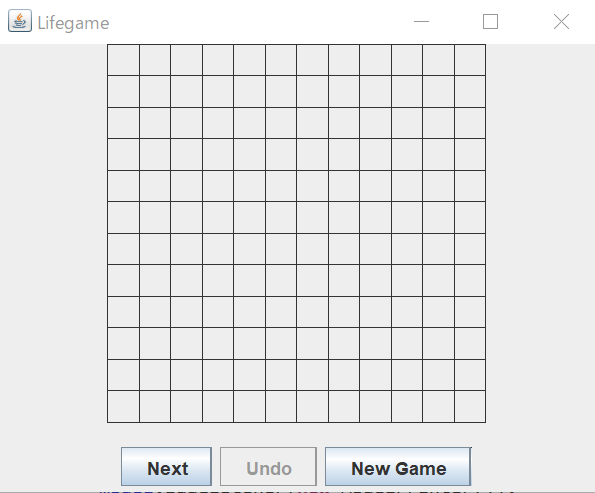
\includegraphics[keepaspectratio, scale=0.4]{panel_normal.png}
    \caption{$12\times12$の盤面}
  \end{minipage}
  \begin{minipage}[b]{0.45\linewidth}
    \centering
    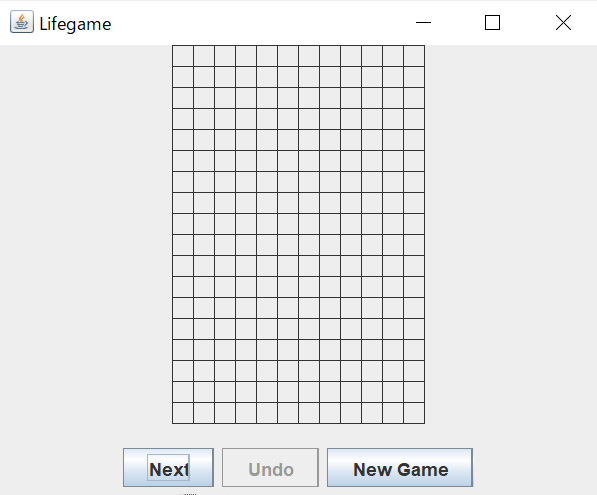
\includegraphics[keepaspectratio, scale=0.4]{1812.png}
    \caption{$18\times12$の盤面}
  \end{minipage}
\end{figure}
\subsection{next,undo,newgameボタン}
ユーザは盤面の下部に表示されるそれぞれのボタンの上にマウスカーソルを移動し左クリックを押し込むことで以下の仕様を満たす処理を実行することができる.
それぞれの処理は左クリックを押し込んで離したときに実行される.
\subsubsection{nextボタン}
nextボタンは最初から押せる状態になっており,ライフゲームの仕様に基づいて世代を一世代進める.
以下の図6,7はnextボタンを押して盤面の状態を一世代進めたときの例である.
\begin{figure}[htbp]
  \begin{minipage}[b]{0.45\linewidth}
    \centering
    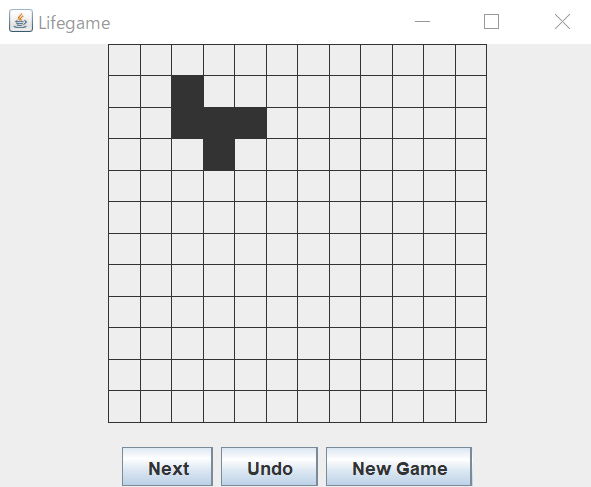
\includegraphics[keepaspectratio, scale=0.35]{before_next.png}
    \caption{nextボタンを押す前の盤面}
  \end{minipage}
  \begin{minipage}[b]{0.45\linewidth}
    \centering
    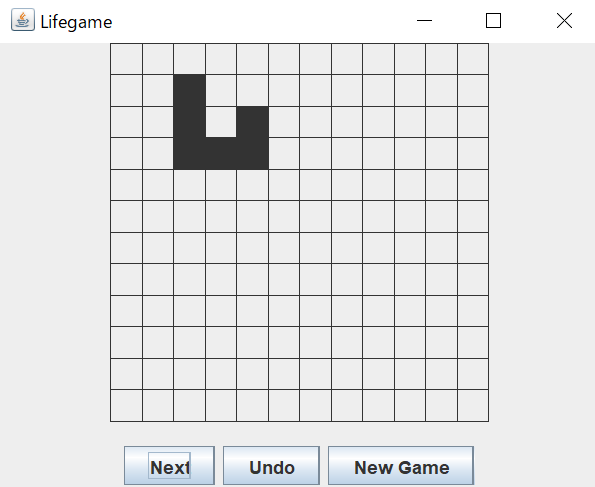
\includegraphics[keepaspectratio, scale=0.35]{after_next.png}
    \caption{nextボタンを押した後の盤面}
  \end{minipage}
\end{figure}
\subsubsection{undoボタン}
undoボタンは最初は押せない状態になっている.nextボタンを押して盤面の状態を1世代進めるか,マウスカーソルを使って盤面内をクリックまたはドラッグした時に押せるようになる.
最大で32の状態を記憶しておき,33回以上盤面の状態が変化した場合は直近の32個の盤面の状態を記憶しておく.
盤面の履歴がこれ以上ない状態まで巻き戻されると再び無効な状態に戻る.したがって,33回盤面の状態が変化した際は,32回undoを押した段階でundoが押せなくなってしまう.
また,盤面の状態の記憶は1セルの状態が変化すると実行されるので,3セル分ドラッグ操作をした場合はその操作で3つの状態が記憶されることになる.
以下の図8はRUNボタンを押したときにUndoボタンが押せなくなっている様子である.
\begin{figure}[h]
  \centering
  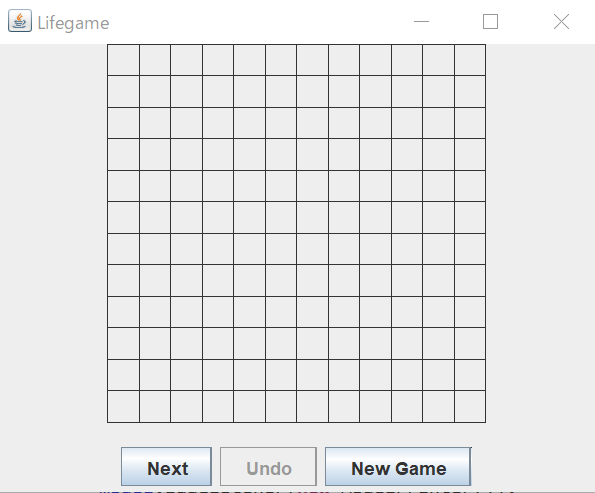
\includegraphics[width=4cm]{panel_normal.png}
  \caption{Undoボタンが押せない様子}
\end{figure}
\\また,以下の図9,10はundoボタンを押して盤面の状態を一世代前に戻したときの例である.
\begin{figure}[htbp]
  \begin{minipage}[b]{0.45\linewidth}
    \centering
    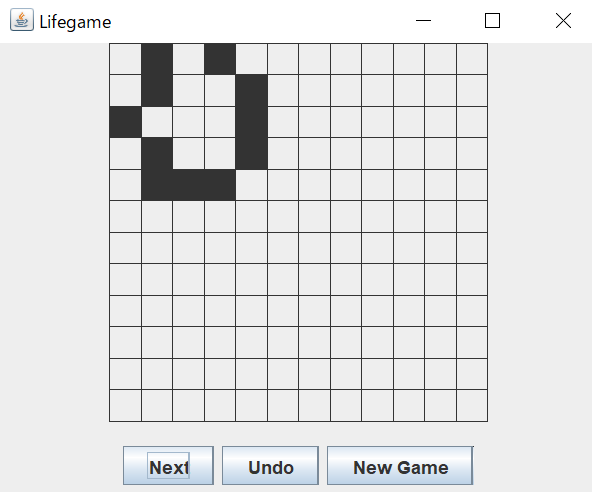
\includegraphics[keepaspectratio, scale=0.35]{before_undo.png}
    \caption{undoボタンを押す前の盤面}
  \end{minipage}
  \begin{minipage}[b]{0.45\linewidth}
    \centering
    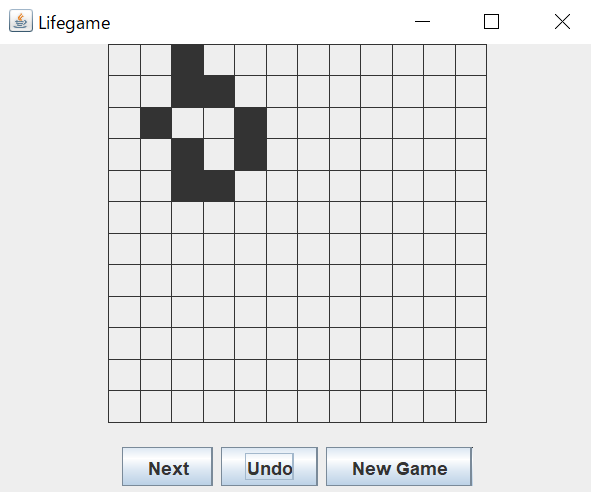
\includegraphics[keepaspectratio, scale=0.4]{after_undo.png}
    \caption{undoボタンを押した後の盤面}
  \end{minipage}
\end{figure}
\subsubsection{newgameボタン}
newgameボタンは最初から押せる状態になっており,ボタンを押すごとに新しく初期化されている盤面を新しいウィンドウで開く.新しく作られたウィンドウはもともとあったウィンドウが作成された位置に作成される.ゲームはそれぞれ
独立しており,片方の盤面の状態を変化させてももう片方の盤面には影響されない.
以下の図11はnewgameボタンを押して新しくウィンドウを開き,片方の盤面にだけマウスカーソルによって状態を変化させた様子である.
\begin{figure}[h]
  \centering
  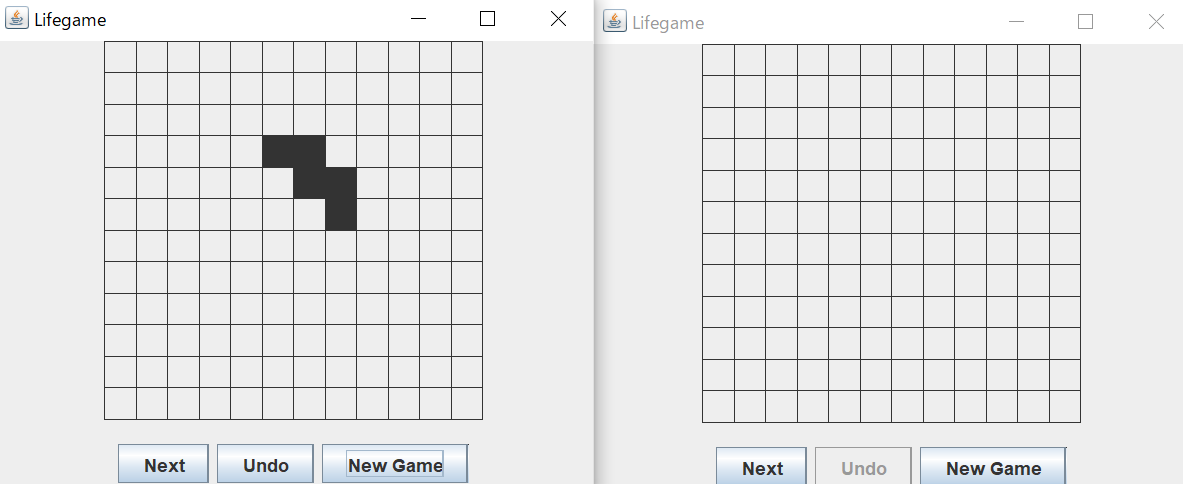
\includegraphics[width=6cm]{newgame.png}
  \caption{newgameボタンを押して片方の盤面だけ変化させた様子}
\end{figure}
\subsection{クリック,ドラッグしたときの処理}
これから記述するクリック操作はマウスカーソルを動かさないで左クリックをすると実行できる.この操作はボタンが押し込まれた瞬間に実行される.
また,ドラッグ操作は左クリックを押し込みながらマウスカーソルを移動させると実行できる.これもクリック操作と同様に,ボタンが押し込まれた瞬間に実行される.
\subsubsection{盤面内のクリック,ドラッグ}
上述のクリック操作により,現在の盤面の状態は反転する.例えば,もともと死んでいる状態のセルをクリックすると生きている状態のクリックに変更し,生きている状態のセルをクリックすると死んでいる状態に変更する.
以下の図12,13は実行例である.この例では(4,3)のセルの状態を反転させている.
\begin{figure}[htbp]
    \begin{minipage}[b]{0.45\linewidth}
      \centering
      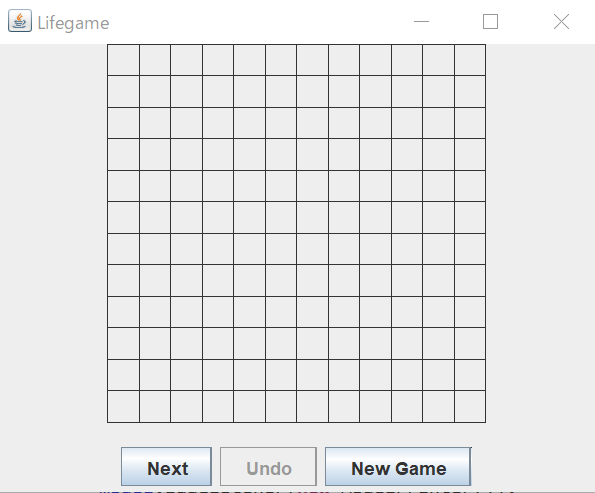
\includegraphics[keepaspectratio, scale=0.4]{panel_normal.png}
      \caption{クリック前の盤面}
    \end{minipage}
    \begin{minipage}[b]{0.45\linewidth}
      \centering
      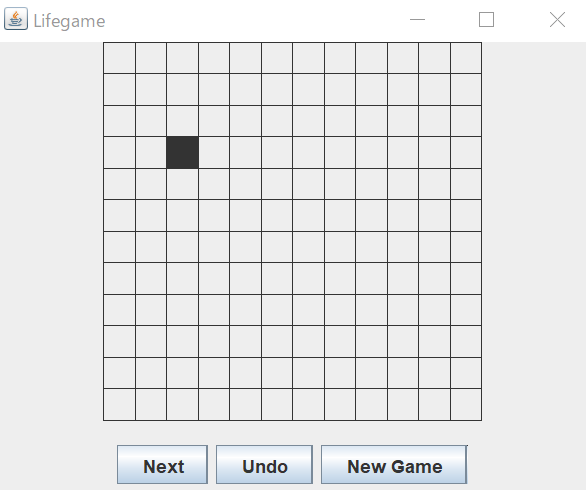
\includegraphics[keepaspectratio, scale=0.4]{panel_click.png}
      \caption{クリックした後の盤面}
    \end{minipage}
  \end{figure}
  \\上述のドラッグ操作により,マウスカーソルがドラッグを開始したセル以外のセルに侵入した
  直後にそのセルの状態が変更される.ただし,同じセル内を移動するだけだと結果としてはクリック操作と同じように押し込んだセルの状態を変更しただけとなる.
  以下の図14,15はドラッグをした時の動作の例である.
  \begin{figure}[htbp]
    \begin{minipage}[b]{0.45\linewidth}
      \centering
      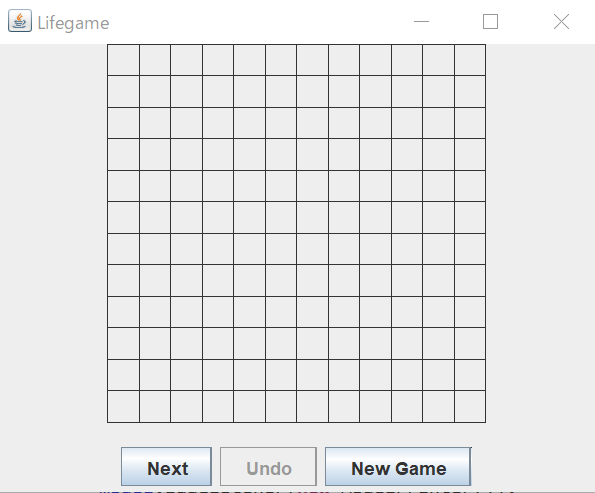
\includegraphics[keepaspectratio, scale=0.4]{panel_normal.png}
      \caption{ドラッグ前の盤面}
    \end{minipage}
    \begin{minipage}[b]{0.45\linewidth}
      \centering
      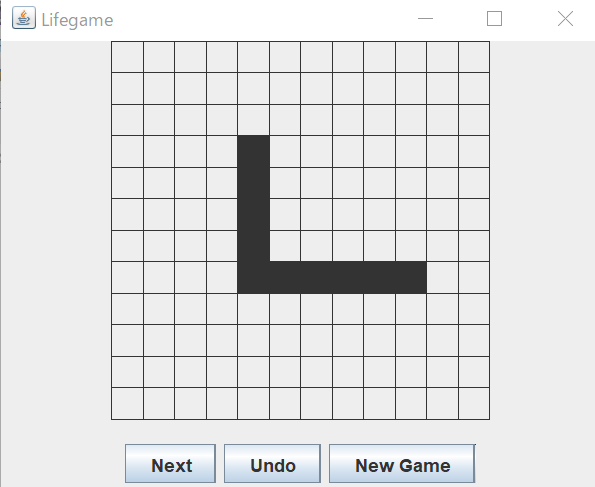
\includegraphics[keepaspectratio, scale=0.4]{panel_drag.png}
      \caption{ドラッグ後の盤面}
    \end{minipage}
\end{figure}
\subsubsection{ドラッグ中にマウスカーソルが盤面以外に移動したときの処理}
盤面外にマウスカーソルを移動させた場合には何も変化が起こらないという仕様にした.また,図16のようにドラッグしながらマウスカーソルを移動させた場合,侵入された盤面の状態のみを変更するので右の図17のように盤面が変更される.
\begin{figure}[htbp]
  \begin{minipage}[b]{0.45\linewidth}
    \centering
    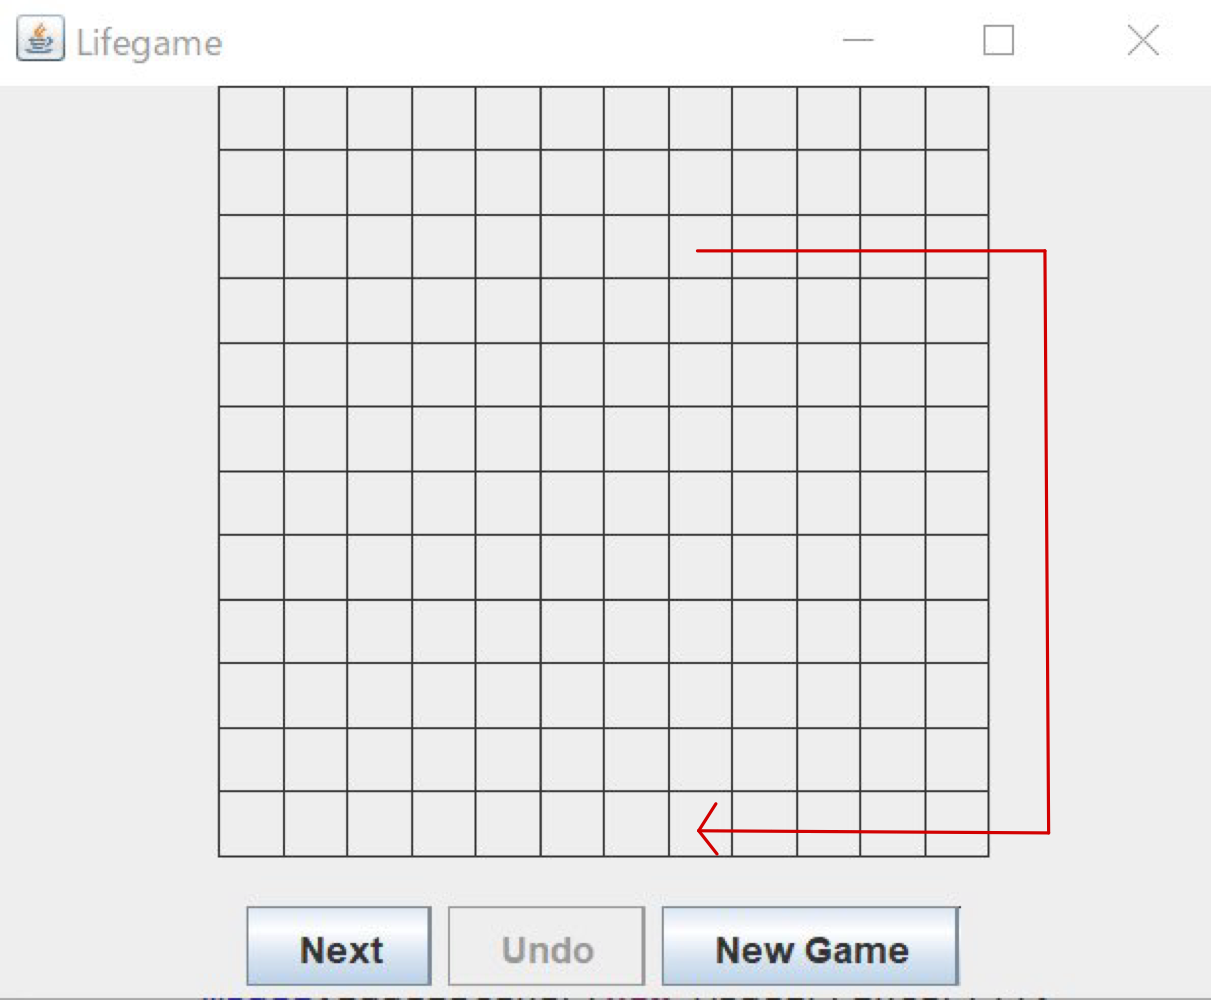
\includegraphics[keepaspectratio, scale=0.1]{tegaki.png}
    \caption{マウスカーソルの動かし方}
  \end{minipage}
  \begin{minipage}[b]{0.45\linewidth}
    \centering
    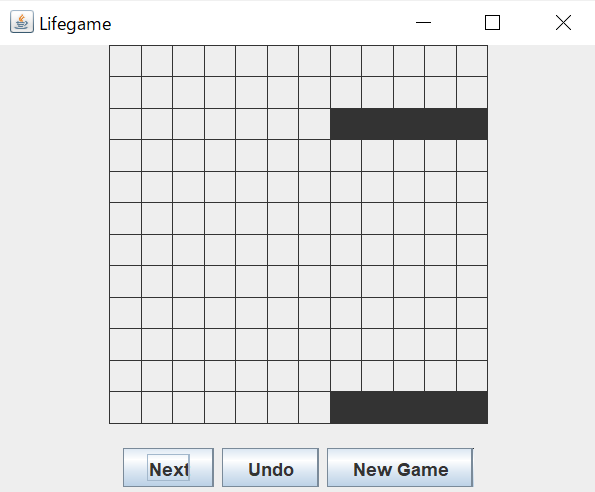
\includegraphics[keepaspectratio, scale=0.4]{after_drag.png}
    \caption{ドラッグ後の盤面}
  \end{minipage}
\end{figure}
\subsubsection{盤面以外をクリックしたときの処理}
盤面以外の場所をクリックした際はドラッグの時と同様に何も起こらないという仕様にした.
\subsubsection{ドラッグ,クリック時のundoボタンの巻き戻し}
1.1.2で記述したundoボタンはクリック,ドラッグ操作による状態の変更も記憶して巻き戻すという仕様とした.ドラッグ操作に関しては,各セル一つずつが状態変化するたびに
新しく盤面が記憶される.

\section{クラスと機能の対応表}
今回作成したライフゲームのプログラムのクラスと機能の対応表は以下のようになる.
\begin{table}[h]
  \centering
  \begin{tabular}{|c|c|}
    \hline
    クラス名&機能\\\hline\hline
    Mainクラス&パネル内の情報の初期設定\\\hline
    BoardModelクラス&盤面の描画と世代更新,巻き戻し処理\\\hline
    Buttonクラス&パネルのボタンが押された時の処理の分類\\\hline
    Boardlistenerインターフェース&盤面の情報\\\hline
    BoardViewクラス&マウスカーソルによる操作\\\hline
  \end{tabular}
  \caption{クラスと機能の対応表}
\end{table}


\section{各機能実装方法}

\subsection{状態の更新に連動して画面表示の変更}
今回のライフゲームでの画面表示が変更されるのは以下のような条件の時である.
\begin{itemize}
    \item nextボタンやundoボタンによる盤面の更新及び巻き戻し
    \item マウスカーソルによる盤面の状態の変更
    \item 
\end{itemize}
これらの処理が行われた後に盤面が再描写されるための処理について記述する.\\
以下のコードはこの処理を実装するためにそれぞれのクラスから必要な個所のみを抜粋したコードである.
\begin{lstlisting}[caption=BoardListenerインターフェース,label=fuga]
    public interface BoardListener {
	    public void updated(BoardModel m);
    }
\end{lstlisting}
\begin{lstlisting}[caption=Mainクラス,label=fuga]
    model.addListener(new BoardView(model));
\end{lstlisting}
\begin{lstlisting}[caption=BoardViewクラス,label=fuga]
    public BoardView(BoardModel model) {
		this.model = model;
		this.addMouseListener(this);
		this.addMouseMotionListener(this);
		model.addListener(this);
	}
    @Override
	public void updated(BoardModel model) {
		this.repaint();
	}
\end{lstlisting}
\begin{lstlisting}[caption=BoardModelクラス,label=fuga]
    private ArrayList<BoardListener> listeners;

    public BoardModel(int c,int r,JButton undoButton) {
		listeners = new ArrayList<BoardListener>();
	}

    public void changeCellState(int x,int y) {
		this.fireUpdate();
	}

    public void addListener(BoardListener listener) {
		listeners.add(listener);
	}
	
	private void fireUpdate() {
		for(BoardListener listener:listeners) {
			listener.updated(this);
		}
	}
\end{lstlisting}
listing1の2行目において,BoardListenerインターフェースにはupdatedクラスが呼び出されている.このupdatedクラスの処理内容はlisting3の8から10行目のように,上で挙げた盤面が更新されるための
処理を実装するクラス内に記述されている.
listing2のコードにより,BoardListenerインターフェースをimplementしたクラスのオブジェクトをlisting4の10から12行目のaddListenerクラスで可変長配列
listenersに登録している.これを行うことで,盤面を変更する各操作が実行されるたびにlisting4の9から12行目のChangeCellStateメソッドが呼び出されて盤面を変更し,その後で18から21行目のfireupdatedメソッドが
呼び出されてrepaintが実行される.これにより,すべての盤面の変更が起こったときにlistenersに登録されたオブジェクトを使ってBoardListenerを介して盤面の再描画が実行される.


\subsection{巻き戻しのための盤面の記憶}
巻き戻しのための盤面の記憶に関する処理はBoardModelクラスに記述した.盤面の情報は可変長配列を持つリスト型であるArraylistを使用し,変数名はHistoryとした.
\subsubsection{nextによる盤面の状態の変更の記憶}
以下のlistingはBoardModelクラスのnextメソッドの一部である.
\begin{lstlisting}[caption=nextメソッドの一部,label=fuga]
    if(counter!=32) {
        counter++;
        History.add(copiedcells);
    }else {
        History.remove(0);
        History.add(copiedcells);
    }
\end{lstlisting}
counterはHistoryに記憶されている状態の数を表すint型の変数で0に初期化されている.counterはメンバであるためcounterの値はほかのメソッドにも共有される.記憶されている状態の数が32個以下ならcounterの値を1インクリメントしてからaddメソッドを使ってHistoryに
状態を記憶し,32個ならHistoryに記憶されている一番古い状態を削除してからaddメソッドを使って現在の状態を新しく記憶している.また,copiedcellsはlifegameの仕様に基づいて一世代進めたあとの盤面の状態を表す二次元配列である.
これは現在の盤面の状態を表す二次元配列cellsのすべての要素をコピーしたものである.copiedcellsを使用している理由としては,次の世代へ進めたときに各セルが生きているかはセルの周りに生きているセルが何個存在するかで決定されるので全てのcellsの要素に参照している途中でcellsの状態を変えてしまうと
周りに存在する生きているセルの数が変化してしまうためである.
\subsubsection{undoによる盤面の状態の変更の記憶}
以下のlistingはBoardModelクラスのundoメソッドの一部である.
\begin{lstlisting}[caption=undoメソッドの一部,label=fuga]
    History.remove(counter);
    counter--;
    cells = History.get(counter);
\end{lstlisting}
まず一番最新の状態をHistoryから削除し,そのあとにcounterを1デクリメントする.これによりundoが押された際に記憶されていた状態が1つ減少する.その後現在の状態を表す二次元配列cells
にデクリメントした後のcounterがさすHistoryの最新の状態,即ちundoを押したときの直前の状態を格納する.
\subsubsection{マウスカーソルによる盤面の状態の変更の記憶}
以下のlistingはBoardModelクラスのchangeCellStateメソッドの一部である.
\begin{lstlisting}[caption=changeCellStateメソッドの一部,label=fuga]
    boolean[][] currentBoard = new boolean[rows][cols];
    for (int i = 0; i < rows; i++) {
        System.arraycopy(cells[i], 0, currentBoard[i], 0, cols);
    }
    if(counter!=32) {
        counter++;
        History.add(currentBoard);
    }else {
        History.remove(0);
        History.add(currentBoard);
    }
\end{lstlisting}
マウスカーソルによる盤面の状態の変更の詳細は後述するが,どのセルの状態を変更すればよいかを特定してから
changeCellStateを呼び出して実際に盤面の状態を格納しているcellsを変更する.二次元配列であるcurrentBoardを用意して変更後の盤面の状態を2から4行目でコピーする.
その後counterの値が32以下ならcounterの値を1インクリメントしてからaddメソッドを使ってHistoryに
状態を記憶し,32個ならHistoryに記憶されている一番古い状態を削除してからaddメソッドを使って現在の状態を新しく記憶している.
addした配列がcellsではなくcurrentBoardである理由は,cellsを格納してしまうと参照の追加になり,cellsが変更されるとHistoryに追加されているほかのオブジェクトも同じように変更されてしまうためである.
ゆえに一時的にcellの内容を別の二次元配列にコピーして参照の追加となることを避けた.
\subsection{undoによる巻き戻し可能かどうかの判定}
undoは盤面を生成したときMainメソッド内でsetEnabledメソッドを使って押せないように初期化されている.undoによる巻き戻しが可能となるのは仕様でも説明した通り
nextボタンによる世代の更新かマウスカーソルによる盤面の状態の変更が行われた時である.
\begin{itemize}
    \item nextボタンによって世代更新が行われた時,3.2.1で記述したようにcounterの値が更新された回数だけインクリメントされる.これを利用してBoardModelメソッド内にisUndoableメソッドを作成した.
    このメソッドはcounterの値が0より大きいときはtrueを,0のときはfalseを返す.以下のlistingのコードはButtonクラス内のnextボタンとundoボタンが押された時に実行される処理である.
    \begin{lstlisting}[caption=nextボタン及びundoボタンを押したときに実行される処理,label=fuga]
        case 1:
            boardModel.next();
            undoButton.setEnabled(true);
            break;
        case 2:
            if(boardModel.isUndoable()) {
                boardModel.undo();
                if(!boardModel.isUndoable()) {
                    undoButton.setEnabled(false);
                }
            }
            break;
    \end{lstlisting}
    1から4行目のように,nextボタンが押された時にはnextメソッドを呼び出して盤面の世代を更新してからsetEnabledメソッドでundoボタンを押せるようにしている.また,6から11行目のように
    isUndoableの返り値がtrueの時はundoメソッドを呼び出して盤面の世代を一つ戻した後に再びisUndoableメソッドを呼び出して返り値がfalseであればsetEnabledメソッドでundoボタンを押せなくしている.
    これは,undoメソッドによって世代を戻したときにHistoryが空になったことをすぐに確認するためである.これを実装することでUndoボタンが履歴がなくなった時に押せなくなることを実現できる.
    \item マウスカーソルによって盤面に変更が加えられたときは仕様で述べた通り,セルの状態が一つでも変わるとそれが一つの盤面の状態として記憶される.3.2.3で記述した通り,マウスカーソルで状態が変更されると
    changeCellStateメソッドが呼び出されるのでこのメソッドが呼び出された時にsetEnabledメソッドでundoボタンを押せるようにすれば巻き戻しを可能にすることが実現できる.
\end{itemize}

\subsection{セルの境界線の位置を計算する方法}
以下の表2は計算するために使用した変数名と表す内容である.
\begin{table}[h]
\centering
\begin{tabular}{|c||c|}
    \hline
    変数名 & 変数があらわす内容\\
    \hline\hline
    M & 盤面の横のセル数\\\hline
    N & 盤面の縦のセル数\\\hline
    width & パネルの横幅\\\hline
    height & パネルの縦幅\\\hline
    masu & 盤面に描写する正方形のマスの一辺の長さ\\\hline
\end{tabular}
\caption{計算式中の変数名とその内容}
\end{table}
\\盤面のセルの境界線の位置は以下のような手順で盤面の境界線の位置は計算される.
\begin{enumerate}
    \item 現在のwidthとheightから,masuを決定する.具体的には以下のような不等式が成り立つかどうかについて考える.
    \begin{align}
        \frac{height\times\frac{99}{100}}{N} > \frac{width}{M+2}
    \end{align}
    左辺はheightの99\%の大きさをN等分した時の長さを調べている.これは,heightの99\%の長さを考えないと盤面の一番下の横線が表示されないことがあるという問題を解決するための処理である.
    右辺はwidthをM+2等分したときの長さを調べている.これは,パネルの中央に盤面を配置するための処理である.(1)が成り立った時はパネルが縦に長い状態であると判断して
    \begin{align}
        masu=\frac{width}{M+2}
    \end{align}
    とし,(1)が成り立たなかったときはパネルが横に長い状態であると判断して
    \begin{align}
        masu = \frac{height\times\frac{99}{100}}{N}
    \end{align}
    となるようにした.
    \item 次に,盤面の開始位置を決定する.縦軸の開始位置はy座標が0からである.x座標の開始位置はパネルの中央に盤面を配置するために,以下のような数式の値を開始位置とする.
    \begin{align}
        \frac{width-masu\times M}{2}
    \end{align}
    この数式はパネルの横幅から盤面を表示している部分の長さを引いた長さを二等分した値になる.これにより,盤面を描写していない部分の横幅が同じ長さとなっている.
    \item ユーザが指定したセル数分だけ縦軸と横軸を描画する.それぞれのセルの一片の長さは(2)または(3)の値である.
\end{enumerate}

\subsection{マウスカーソルの座標からセルの座標を計算する方法}
以下の表3は計算するために使用した変数名と表す内容である.
\begin{table}[h]
    \centering
    \begin{tabular}{|c||c|}
        \hline
        変数名 & 変数があらわす内容\\
        \hline\hline
        M & 盤面の横のセル数\\\hline
        N & 盤面の縦のセル数\\\hline
        width & パネルの横幅\\\hline
        height & パネルの縦幅\\\hline
        masu & 盤面に描写する正方形のマスの一辺の長さ\\\hline
        x & マウスカーソルがある場所のx座標\\\hline
        y & マウスカーソルがある場所のy座標\\\hline
        masu\_x & 0で初期化されており,マウスカーソルが現在存在するセルの左上の頂点のx座標\\\hline
        masu\_y & 0で初期化されており,マウスカーソルが現在存在するセルの左上の頂点のy座標\\\hline
        StateX & マウスカーソルが現在存在するセルの左上の頂点のx座標\\\hline
        StateY & マウスカーソルが現在存在するセルの左上の頂点のy座標\\\hline
    \end{tabular}
    \caption{計算式中の変数名とその内容}
    \end{table}
\\3.4の表2の変数と同じ変数名のものは値も同じである.以下のような流れでマウスカーソルがある位置のセルの座標はクリックとドラッグで異なる方法で計算される.
まずクリックとドラッグで共通の処理を記述する.
盤面外にマウスカーソルがある状態でクリックやドラッグがされると何もしないようにするためにxとyが以下の条件式を満たしているか確認する.
\begin{align}
    x < \frac{width-masu\times M}{2} \quad or \quad x> \frac{width+masu\times M}{2}\quad or \quad y > masu\times (N)
\end{align}
これらの3つの不等式の一番左の不等式はマウスカーソルのx座標が盤面よりも左側にあるとき真になる.真ん中はマウスカーソルのx座標が盤面よりも右側にあるとき真になる.
一番右の不等式はマウスカーソルのy座標が盤面よりも下側にある時に真になる.そしてこれら3つの不等式は全てorとしているのでこれらのうちの1つでも真になれば盤面外にマウスカーソルがあるという判定になる.
\subsubsection{クリック時の計算}
クリック時のマウスカーソルの位置からのセルの座標の計算は以下のような流れで実行される.
\begin{enumerate}
    \item 
\end{enumerate}
\subsection{マウスカーソルによる盤面の状態の変更}

  マウスカーソルによる盤面の状態の変更に関する処理はBoardViewクラスに記述した.以下にクリックに関する処理とドラッグに関する処理の実装方法を記述する.
この処理を行うにあたって使用したメンバは以下のとおりである.

\begin{table}[h]
    \centering
    \begin{tabular}{|c||c|}
        \hline
        変数名 & 変数があらわす内容\\
        \hline\hline
        width & パネルの横幅をpaintメソッド内のgetWidthメソッドによって格納するint型の変数 \\\hline
        height & パネルの縦幅をpaintメソッド内のgetHeightメソッドによって格納するint型の変数\\\hline
        masu & 盤面に描写する正方形のマスの一辺の長さを格納するint型の変数\\\hline
        M & 盤面の横のマス数\\\hline
        N & 盤面の縦のマス数\\\hline
        StateX & マウスカーソルが現在存在するセルの左上の頂点のx座標を格納するint型の変数\\\hline
        StateY & マウスカーソルが現在存在するセルの左上の頂点のy座標を格納するint型の変数\\\hline
    \end{tabular}
    \caption{メンバとその内容}
\end{table}
また,masuの計算は2.3で記述した通りである.

\begin{description}
    \item [クリック時の処理]\mbox{}\\
    クリック時の処理はmousepressedメソッド内に記述した.
    mousepressedメソッド内で使用する内部変数は以下のとおりである.
    \begin{table}[h]
        \centering
        \begin{tabular}{|c||c|}
            \hline
            変数名 & 変数があらわす内容\\\hline\hline
            x & マウスカーソルがある場所のx座標を格納するint型の変数\\\hline
            y & マウスカーソルがある場所のy座標を格納するint型の変数\\\hline
            i &for文を使う際のカウンタ\\\hline
            j &for文を使う際のカウンタ \\\hline
        \end{tabular}
        \caption{内部変数名とその内容}
    \end{table}
    クリック操作時の具体的な処理内容は以下のような流れで実行される.
    \begin{enumerate}
        \item x,yの宣言及び初期化をする.x,yはgetcol関数により取得される.
        \item マウスカーソルが盤面内に存在するかどうかを判定し,存在すれば3以降の処理を実行する.存在しなければクリックの処理をreturn文により終了する
        \item for文を使って今現在のマウスカーソルが存在する座標のセルのy座標を特定.このとき,特定するための条件式$y>=i*masu \&\& y<(i+1)*masu$は,カウンタを表す変数iによって盤面のセルのどの行にyが存在するかを判定している.
        \item 3でyがどの行にあるかを特定した後,同様にしてxがどの列にあるのかを判定する.条件式は$x>=\frac{(wodth-masu*M)}{2}+masu*j\&\& x<\frac{width-masu*M}{2}+masu*(j+1)$となる.2の条件式との違いは,盤面を描写し始める位置が異なるためである.
        \item StateXとStateYを3と4で条件分岐をした時のiとjを使ってマウスカーソルが存在するセルの左上の頂点の座標を格納する.これは,後のドラッグ操作ための処理であるため後に記述する.そのあとbreak文を二回使ってfor文から抜ける.
        \item 特定したiとjをchangeCellStateメソッドの引数として使用しセルの状態を変える.そしてpaintメソッドを使って盤面を描写する.
    \end{enumerate}
    \item [ドラッグ時の処理]\mbox{}\\
    ドラッグ時の処理はmouseDraggedメソッド内に記述した.
    mouseDraggedメソッド内で使用する内部変数は以下のとおりである.
    \begin{table}[h]
        \centering
        \begin{tabular}{|c||c|}
            \hline
            変数名 & 変数があらわす内容\\\hline\hline
            x & マウスカーソルがある場所のx座標を格納するint型の変数\\\hline
            y & マウスカーソルがある場所のy座標を格納するint型の変数\\\hline
            masu\_x & 0で初期化されており,マウスカーソルが現在存在するセルの左上の頂点のx座標を格納するint型の変数\\\hline
            masu\_y & 0で初期化されており,マウスカーソルが現在存在するセルの左上の頂点のy座標を格納するint型の変数\\\hline
            i &for文を使う際のカウンタ\\\hline
            j &for文を使う際のカウンタ \\\hline
        \end{tabular}
        \caption{内部変数名とその内容}
    \end{table}
    クリック操作時の具体的な処理内容は以下のような流れで実行される.
    \begin{enumerate}
      \item クリック時の処理の1から4と同様の処理が行われる.また,最初にmasu\_xとmasu\_yを0で初期化する.
      \item StateXとStateYではなく,masu\_xとmasu\_yに特定したi,jを使ってxとyが存在するセルの左上の頂点の座標を格納する.
      \item masu\_xとmasu\_yがそれぞれStateXとStateYと一致しているかを判定する.即ち直前にマウスカーソルがあったセルと今現在マウスカーソルが存在しているセルが一致しているかどうかを判定している.
      一致していれば何も処理をせずに終了し,一致していなければ以下の4の処理を行う.
      \item for文を二回使用してクリック時のStateXやStateYを求めた時と同じようにchangeCellStateメソッドとrepaintメソッドを使って変更された盤面を表示する.
    \end{enumerate}
    ドラッグ操作では,クリック操作とは違って現在のセルの位置を格納する変数としてmasau\_Xとmasu\_yを使用した.これは,ドラッグ操作をする際に同じマス中の移動の際に盤面の状態が何度も変更されて最初の状態が維持されないという問題が発生したからであるb.
    これを解決するために直前の状態を保存しておくことで同じセル内を移動するときには盤面の状態を変化させないようにした.
\end{description}

\subsection{新しいウィンドウを開く}
新しいウィンドウを開くことに関する処理はクラスのメソッドに記述した.
この処理を行うにあたって使用したメンバは以下のとおりである.
\begin{table}[h]
  \centering
  \begin{tabular}{|c||c|}
    \hline
    変数名 & 変数があらわす内容\\
    \hline\hline
    M & 盤面の横のマス数\\\hline
    N & 盤面の縦のマス数\\\hline
    width & パネルの横幅をpaintメソッド内のgetWidthメソッドによって格納するint型の変数 \\\hline
    height & パネルの縦幅をpaintメソッド内のgetHeightメソッドによって格納するint型の変数\\\hline
    masu & 盤面に描写する正方形のマスの一辺の長さを格納するint型の変数\\\hline

  \end{tabular}
  \caption{メンバとその内容}
\end{table}



\subsection{拡張機能}


\subsubsection{実現方法}


\section{プログラミングの講義・演習で学習したこと}


\subsection{演習前から知っていたこと}

私は大学生になるまでプログラミングの経験がなく,大学のプログラミングの講義等でしか触れる機会が無かった.そのため,今回の講義・演習で初めてオブジェクト指向言語について学習した.
以前からオブジェクト指向プログラミングというものの存在は認知していたが,プログラミング歴の浅い自分にとっては難易度が高く思えていた.
\end{document}